\documentclass[a4paper,12pt]{article}


\usepackage[english]{babel}
\usepackage[T1]{fontenc}
\usepackage[toc,page]{appendix}
\usepackage{amssymb}
\usepackage{amsmath}
\usepackage{latexsym}
\usepackage{graphicx}
\usepackage{beramono}% monospaced font with bold variant

\usepackage{listings}
\lstdefinelanguage{VHDL}{
	morekeywords={
		PORT,END COMPONENT,IN,OUT,in,out,COMPONENT,component,port,end component,library,use,all,entity,is,port,in,out,end,architecture,of,
		begin,and, std_logic_vector, shift_right,signed, end if, end process,if,else,process,not,after,wait
	},
	morecomment=[l]--
}

\usepackage{xcolor}
\colorlet{keyword}{blue!100!black!80}
\colorlet{comment}{green!90!black!90}
\lstdefinestyle{vhdl}{
	language     = VHDL,
	basicstyle   = \ttfamily,
	keywordstyle = \color{keyword}\bfseries,
	commentstyle = \color{comment}
}



\setlength{\parindent}{0pt}
\begin{document}
\section*{MAPD FPGA Lab 7 - Homework Report}
Vincenzo Maria Schimmenti 1204565\\

\begin{figure}[h!]
	\begin{flushleft}
		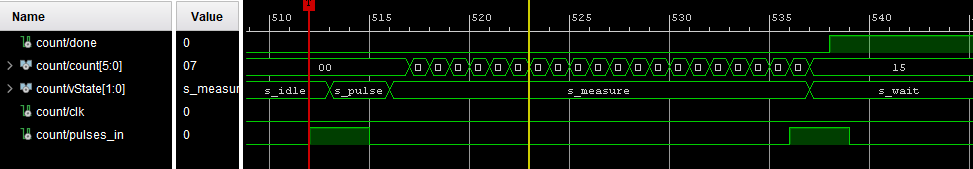
\includegraphics[width=1.2\linewidth,keepaspectratio]{Cattura.png}
	\end{flushleft}	
	\caption{ILA result}
	\label{fig:fir5ex}
\end{figure}

\begin{lstlisting}[style=vhdl]
library IEEE;
use IEEE.STD_LOGIC_1164.ALL;

-- Uncomment the following library declaration if using
-- arithmetic functions with Signed or Unsigned values
use IEEE.NUMERIC_STD.ALL;

-- Uncomment the following library declaration if instantiating
-- any Xilinx leaf cells in this code.
--library UNISIM;
--use UNISIM.VComponents.all;

entity break_measure is
generic(DONE_TIME : integer := 100);
Port (clk   : in  std_logic;
rst   : in  std_logic;            
pulses_in  : in  std_logic; -- Counter input
count_out  : out unsigned(5 downto 0); -- break time measurement in clock cycles
done_out   : out std_logic);-- Calculation done
end break_measure;

architecture Behavioral of break_measure is

COMPONENT ila_0

PORT (
clk : IN STD_LOGIC;

probe0 : IN STD_LOGIC_VECTOR(0 DOWNTO 0);
probe1 : IN STD_LOGIC_VECTOR(5 DOWNTO 0);
probe2 : IN STD_LOGIC_VECTOR(1 DOWNTO 0);
probe3 : IN STD_LOGIC_VECTOR(0 DOWNTO 0);
probe4 : IN STD_LOGIC_VECTOR(0 DOWNTO 0)
);
END COMPONENT  ;

type bm_state is (s_idle, s_pulse, s_measure,s_wait); 
signal bms : bm_state;
signal count : STD_LOGIC_VECTOR(5 downto 0);
signal done : std_logic;
signal vState : std_logic_vector(1 downto 0);
begin

ila0 : ila_0
PORT MAP (
clk => clk,
probe0(0) => done,
probe1 => count,
probe2 => vState,
probe3(0) => clk,
probe4(0) => pulses_in
);

bm_fsm : process(clk, rst, pulses_in) is
variable cnt : integer;
variable wcnt : integer;
begin
if rst = '1' then
bms <= s_idle;
cnt := 0;
wcnt := 0;
done <= '0';
elsif rising_edge(clk) then
case bms is
when s_idle => --pretty sure it's correct
if pulses_in ='1' then --first pulse about to start
bms <= s_pulse;
else
bms <= s_idle; 
end if;
when s_pulse =>
if pulses_in ='0' then --pulse finished
bms <= s_measure;
else
bms <= s_pulse;
end if;
when s_measure =>
if pulses_in ='1' then --measure finished
bms <= s_wait;
else             
bms <= s_measure;
end if;
cnt := cnt + 1;
when s_wait =>
if wcnt < DONE_TIME then
done <= '1';
wcnt := wcnt + 1;
bms <= s_wait;
else
--go back to idle state
done<= '0';
wcnt := 0;
cnt := 0;
bms <= s_idle;
end if;
end case;
end if;
done_out <= done;
vState <= std_logic_vector(to_unsigned(bm_state'pos(bms),2));
count <= std_logic_vector(to_unsigned(cnt, 6));
count_out <= to_unsigned(cnt, 6);
end process;



end Behavioral;

\end{lstlisting}

\end{document}